\documentclass{article}

\usepackage{geometry}
\usepackage{xeCJK}
\usepackage{amsmath}
\usepackage{tikz}
\usepackage{pgfplots}
% figure[H] float
\usepackage{float}
% subfigure
\usepackage{subcaption}
\usepackage{amssymb}
\usepackage{hyperref}
\usepackage{setspace}
% 修改公式编号
\usepackage{chngcntr}
% 提供长等号和文本在等号上方
\usepackage{extarrows}
% 表格单元格对角线:diagbox、pict2e
\usepackage{diagbox}
\usepackage{pict2e}

% 设置行间距 1.5 倍
\renewcommand{\baselinestretch}{1.5}

% 设置页大小和页边距,或者scale=0.8
\geometry{a4paper,left=3.18cm,right=3.18cm,top=2.54cm,bottom=2.54cm}
% 兼容
\pgfplotsset{compat=1.16}
% 中文默认没有斜体和粗体格式,开启伪斜体和指定黑体;
\setCJKmainfont[AutoFakeSlant, BoldFont=SimHei]{SimSun}
\usetikzlibrary{positioning}
\hypersetup{
    colorlinks,
    citecolor=black,
    filecolor=black,
    linkcolor=black,
    urlcolor=black
}
% 每个章节后,重置公式编号
\counterwithin*{equation}{section}
% area of hatch,面积阴影部分
\usetikzlibrary{patterns}

% make cdot thicker,比 cdot 更粗的圆点
\makeatletter
\newcommand*\bigcdot{\mathpalette\bigcdot@{.5}}
\newcommand*\bigcdot@[2]{\mathbin{\vcenter{\hbox{\scalebox{#2}{$\m@th#1\bullet$}}}}}
\makeatother
% 修改公式标签引用颜色
\def\eqref#1{{\color{blue}\hypersetup{linkcolor=blue} (\ref{#1}) }}
% 修改图片标签引用的颜色
\def\figureref#1{{\color{blue}\hypersetup{linkcolor=blue} (\ref{#1}) }}
% 修改跳转标签引用的颜色
\def\linkref[#1]#2{\hyperref[#1]{\color{blue} #2}}

\begin{document}
  \tableofcontents
  \newpage

  \section{概率论的基本概念}
    \subsection{随机试验}
\paragraph{}
\textbf{随机试验}的三个特点,用$E$表示:

\begin{enumerate}
  \item 可以在相同的条件下重复地进行
  \item 每次试验的可能结果不止一个,并且能事先明确试验的所有可能结果
  \item 进行一次试验之前不能确定哪一个结果会出现
\end{enumerate}

\paragraph{}
例子:

\label{s1_1}
\paragraph{}
$E_1$:抛一枚硬币,观察正面$H$、反面$T$出现的情况。

\subsection{样本空间、随机事件}
\subsubsection{样本空间}
\paragraph{}

随机试验$E$的所有可能结果组成的集合称为$E$的\textbf{样本空间},记为$S$,样本空间的元素,即每个结果,称为\textbf{样本点}。

\paragraph{}
例子,\linkref[s1_1]{$E_1$}的样本空间:

\paragraph{}
$S_1: \{H, T\};$

\subsubsection{随机事件}
\paragraph{}
试验$E$的样本空间$S$的子集为$E$的\textbf{随机事件},简称\textbf{事件},当且仅当这一子集中的一个样本点出现时,称这一\textbf{事件发生}。

\paragraph{}
由一个样本点组成的单点集,称为\textbf{基本事件},样本空间$S$包含所有的样本点,它是$S$自身的子集,在每次试验中它总是发生的,$S$称为\textbf{必然事件},空集$\varnothing$在每次试验中都不发生,称为\textbf{不可能事件}。

\subsubsection{事件间的关系与事件的运算}
\paragraph{}
事件是一个集合,符合集合的运算。

\paragraph{}
设试验$E$的样本空间为$S$,而$A, B, A_k(k = 1, 2, \cdots)$是$S$的子集:

\begin{enumerate}
  \item 若$A \subset B$,则事件$B$包含事件$A$,事件$A$发生必导致事件$B$发生。若$A \subset B$ 且 $B \subset A \Rightarrow A = B$,称事件$A$与事件$B$\textbf{相等}。
  \item 事件$A \cup B = \{x | x \in A \; \text{或} \; x \in B\}$称为事件$A$与事件$B$的\textbf{和事件}。${\displaystyle \bigcup_{k=1}^{n}} A_k$为$n$个事件$A_1, A_2, \cdots$的和事件。
  \item 事件$A \cap B=\{x | x \in A \; \text{且} \; x \in B\}$称为事件$A$与事件$B$的\textbf{积事件}。${\displaystyle \bigcap_{k=1}^{n}} A_k$为$n$个事件$A_1, A_2, \cdots$的积事件。
  \item 事件$A-B=\{x | x \in A \; \text{且} \; x \notin B\}$称为事件$A$与事件$B$的\textbf{差事件}。
  \item 若 $A \cap B = \varnothing$,且称事件$A$与$B$是\textbf{互不相容的},或\textbf{互斥的}。
  \item 若 $A \cup B = S$ 且 $A \cap B = \varnothing$,称事件$A$与事件$B$互为\textbf{逆事件},又称\textbf{对立事件},记为$\overline{A} = S - A$。
\end{enumerate}

\paragraph{}
集合中,有些教材,\textbf{差运算}$S - A$用$S \symbol{92} A$表示,\textbf{补集}$\overline{A}$用$A^{c}$表示。

\begin{figure}[H]
\centering
  %------- 第1行 -------
  \begin{subfigure}[t]{0.3\linewidth}
    \centering
      \input{figure/1/A_subset_B}
      \caption{$A \subset B$}
      \label{1_A_subset_B}
  \end{subfigure}
  \begin{subfigure}[t]{0.3\linewidth}
    \centering
      % A 并 B
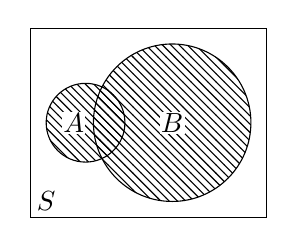
\begin{tikzpicture}
  %---------------- cup ----------------
  \draw (-0.8,0) circle [radius=.5];
  \fill[pattern=north west lines] (-0.8,0) circle [radius=.5];
  \node[fill=white, inner sep=.5] at (-.95,0) {$A$};

  \draw (0.3,0) circle [radius=1];
  \fill[pattern=north west lines] (0.3,0) circle [radius=1];
  \node[fill=white, inner sep=.5] at (0.3,0) {$B$};

  \draw (-1.5,-1.2) rectangle (1.5,1.2);
  \node at (-1.3,-1) {$S$};
\end{tikzpicture}

      \caption{$A \cup B$}
      \label{1_A_cup_B}
  \end{subfigure}
  \begin{subfigure}[t]{0.3\linewidth}
    \centering
      % A 交 B
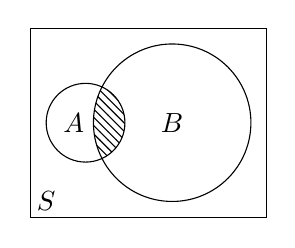
\begin{tikzpicture}
  % circle A
  \draw (-.8,0) circle [radius=.5];
  \node at (-.95,0) {$A$};
  % circle B
  \draw (0.3,0) circle [radius=1];
  \node at (0.3,0) {$B$};
  % A 交 B
  \begin{scope}
    \clip (-.8, 0) circle (.5);
    \clip (0.3, 0) circle (1);
    \fill[pattern=north west lines] (-0.7,-1) rectangle (1.3,1);
  \end{scope}
  % rectangle S
  \draw (-1.5,-1.2) rectangle (1.5,1.2);
  \node at (-1.3,-1) {$S$};
\end{tikzpicture}

      \caption{$A \cap B$}
      \label{1_A_cap_B}
  \end{subfigure}

  \bigskip %------- 第2行 -------
  \begin{subfigure}[b]{0.3\linewidth}
    \centering
      \input{figure/1/A_difference_B}
      \caption{$A - B$}
      \label{1_A_diffence_B}
  \end{subfigure}
  \begin{subfigure}[b]{0.3\linewidth}
    \centering
      % A 交 B = 空集
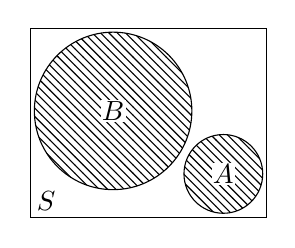
\begin{tikzpicture}

  % circle B
  \draw[pattern=north west lines] (-.45,.15) circle [radius=1];
  \node[fill=white, inner sep=.5] at (-.45,.15) {$B$};

  % circle A
  \draw[pattern=north west lines] (.95,-.65) circle [radius=.5];
  \node[fill=white, inner sep=.5] at (.95,-.65) {$A$};

  \draw (-1.5,-1.2) rectangle (1.5,1.2);
  \node at (-1.3,-1) {$S$};
\end{tikzpicture}

      \caption{$A \cap B = \varnothing$}
      \label{1_A_cap_nothing_B}
  \end{subfigure}
  \begin{subfigure}[b]{0.3\linewidth}
    \centering
      \input{figure/1/B_complement}
      \caption{$B \cup \overline{B} = S; B \cap \overline{B} = \varnothing$}
      \label{1_B_complement}
  \end{subfigure}
  \caption{事件$A$和事件$B$的关系和运算}
  \label{事件A和事件B的关系和运算}
\end{figure}

\subsubsection{常用运算公式}
\paragraph{}
设$A, B, C$为事件,则:

\begin{enumerate}
  \item 交换律:
  \begin{align}
    \begin{split}
    A \cup B = B \cup A; \\
    A \cap B = B \cap A
    \end{split}
  \end{align}
  \item 结合律:
  \begin{align}
    \begin{split}
    A \cup (B \cup C) = (A \cup B) \cup C; \\
    A \cap (B \cap C) = (A \cap B) \cap C
    \end{split}
  \end{align}
  \item 分配律:
  \begin{align}
    \begin{split}
    A \cup (B \cap C) = (A \cup B) \cap (A \cup C); \\
    A \cap (B \cup C) = (A \cap B) \cup (A \cap C)
    \end{split}
  \end{align}
  \item 德摩根律:
  \begin{align}
    \begin{split}
    \overline{A \cup B} = \overline{A} \cap \overline{B}; \\
    \overline{A \cap B} = \overline{A} \cup \overline{B}
    \end{split}
  \end{align}
\end{enumerate}

\subsection{频率与概率}
\subsubsection{频率}
\paragraph{}
\textbf{定义\;}在相同的条件下,进行了$n$次试验,在这$n$次试验中,事件$A$发生的次数$n_A$称为事件$A$发生的\textbf{频数}。比值$n_A / n$称为事件$A$发生的\textbf{频率},记为$f_n(A)$。

\paragraph{}
频率具有下述基本性质:
\begin{enumerate}
  \item $0 \leq f_n(A) \leq 1$
  \item $f_n (S) = 1$
  \item 若$A_1, A_2, \cdots, A_k$是两两互不相容的事件,则
  \begin{equation}
    f_n(A_1 \cup A_2 \cup \cdots \cup A_k) = f_n(A_1) + f_n(A_2) + \cdots + f_n(A_k)
  \end{equation}
\end{enumerate}

\paragraph{}
需要重复大量试验,频率$f_n(A)$呈现稳定性,稳定于某个常数。这种稳定性称为\textbf{统计规律性}。重复大量次数试验,计算频率$f_n(A)$,以它表征事件$A$发生可能性的大小是合适的。

\paragraph{}
实际中,不可能每个事件都可以做大量的试验,因此理论研究通过\textbf{概率}来表征事件发生可能性大小。

\subsubsection{概率}
\paragraph{}
\textbf{定义\;}设$E$是随机试验,$S$是它的样本空间,对于$E$的每一个事件$A$赋予一个实数,记为$P(A)$,称为事件$A$的\textbf{概率},如果集合函数$P(\cdot)$满足:
\begin{enumerate}
  \item \textbf{非负性:}对于每一个事件$A$,有$P(A) \geq 0$
  \item \textbf{规范性:}对于必然事件$S$,有$P(S)=1$
  \item \textbf{可列可加性:}设$A_1, A_2, \cdots$是两两互不相容的事件,即对于$A_iA_j=\varnothing, i \neq j, i, j=1,2,\cdots,$有$ P(A_1 \cup A_2 \cup \cdots)=P(A_1)+P(A_2)+\cdots$
\end{enumerate}

\paragraph{}
推导性质:

\begin{enumerate}
  \item $P(\varnothing) = 0$
  \item \textbf{有限可加性\;}若$A_1, A_2, \cdots, A_n$是两两互不相容的事件,则有$ P(A_1 \cup A_2 \cup \cdots \cup A_n)=P(A_1)+P(A_2)+\cdots+P(A_n)$
  \item 设$A, B$是两个事件,若$A \subset B$,则有:
  \begin{align}
    \begin{split}
    P(B-A) =&\; P(B) - P(A); \\
    P(B) \geq &\; P(A)
    \end{split}
  \end{align}
  \item 对于任一事件$A$,$P(A) \leq = 1$
  \item \textbf{逆事件的概率\;}对于任一事件$A$,有$P(\overline{A}) = 1-P(A)$
  \item \textbf{加法公式\;}对于任意两个事件$A, B$有$P(A \cup B)=P(A)+P(B)-P(AB)$,\\ 一般,对于任意$n$个事件$A_1, A_2, \cdots , A_n$,可用归纳法证得
  \begin{align}
    \begin{split}
    P(A_1 \cup A_2 \cup \cdots \cup A_n) =& \; \sum_{i=1}^{n}P(A_i) - \sum_{1 \leq i < j \leq n}P(A_iA_j) \\
    & \; + \sum_{1 \leq i < j < k \leq n}P(A_iA_jA_k)+ \cdots + (-1)^{n-1}P(A_1A_2 \cdots A_n)
    \end{split}
  \end{align}
\end{enumerate}

\subsection{等可能概型(古典概型)}
\paragraph{}
\textbf{等可能概型\;}的特点:
\begin{enumerate}
  \item 试验的样本空间只包含有限个元素
  \item 试验中每个基本事件发生的可能性相同
\end{enumerate}
\paragraph{}
若事件$A$包含$k$个基本事件,即$A = \{e_{i_1}\} \cup \{e_{i_2}\} \cup \cdots \cup \{e_{i_k}\}$,这里$i_1, i_2, \cdots, i_k$是$1, 2, \cdots, n$中某$k$个不同的数,则:
\begin{equation}
  P(A) = \sum_{j=1}^{k}P(\{e_{i_j}\}) = \frac{k}{n} = \frac{\text{$A$包含的基本事件数}}{\text{$S$中基本事件的总数}}
\end{equation}

\paragraph{}
概率很小的事件在一次试验中实际上几乎是不发生的,称为\textbf{实际推断原理}。
\paragraph{}
\textbf{例\;}某接待站在某一周曾接待过$12$次来访,已知所有这$12$次接待都是在周二和周四进行的,问是否可以推断接待时间是有规定的?
\paragraph{}
\textbf{解\;}假设接待站的接待时间没有规定,而各来访者在一周的任意一天中去接待站是等可能的,那么,$12$次接待来访者都在周二、周四的概率为
\begin{equation*}
  \frac{2^{12}}{7^{12}} = 0.000 \; 000 \; 3
\end{equation*}
\paragraph{}
因此,推断出接待时间是有规定的。

\subsection{条件概率}
\subsubsection{条件概率}
\paragraph{}
\label{条件概率定义}
\textbf{定义\;}设试验的基本事件总数为$n, A$所包含的基本事件数为$m(m>0)$,$AB$所包含的基本事件数为$k$,即:
\begin{equation}
  P(B|A) = \frac{k}{m} = \frac{k/n}{m/n} = \frac{P(AB)}{P(A)},
\end{equation}
称为在事件$A$发生的条件下事件$B$发生的\textbf{条件概率}。
\paragraph{}
条件概率$P(\cdot | A)$符合概率定义中的三个条件:
\begin{enumerate}
  \item \textbf{非负性:}对于每一事件$B$,有$P(B|A)\geq 0$
  \item \textbf{规范性:}对于必然事件$S$,有$P(S|A)=1$
  \item \textbf{可列可加性:}设$B_1, B_2, \cdots$是两两互不相容的事件,则:
  \begin{equation}
    P(\bigcup_{i=1}^\infty B_i | A) = \sum_{i=1}^\infty P(B_i | A),
  \end{equation}
\end{enumerate}
对任意事件$B_1, B_2$有$P(B_1 \cup B_2 | A) = P(B_1 | A) + P(B_2 | A) - P(B_1B_2|A)$

\subsubsection{乘法定理}
\paragraph{}
由\linkref[条件概率定义]{条件概率的定义},可得到下述定理。
\paragraph{}
\textbf{乘法定理\;}设$P(A)>0$,则有
\begin{equation}
  \label{乘法公式}
  P(AB) = P(B|A)P(A)
\end{equation}
\eqref{乘法公式}式称为\textbf{乘法公式}。
\paragraph{}
一般,设$A_1, A_2, \cdots, A_n$为$n$个事件,$n \geq 2$,且$P(A_1A_2\cdots A_{n-1}) > 0$,则有:
\begin{equation}
  P(A_1A_2\cdots A_n) = P(A_n|A_1A_2\cdots A_{n-1})P(A_{n-1}|A_1A_2\cdots A_{n-2})\cdots P(A_2|A_1)P(A_1).
\end{equation}

\subsubsection{全概率公式和贝叶斯公式}
\paragraph{}
\textbf{定义\;}设$S$为试验$E$的样本空间,$B_1, B_2, \cdots, B_n$为$E$的一组事件,若:
\begin{enumerate}
  \item $B_iB_j=\varnothing, i \neq j, i,j = 1,2,\cdots,n$
  \item $B_1 \cup B_2 \cup \cdots \cup B_n = S$
\end{enumerate}
则称$B_1,B_2,\cdots,B_n$为样本空间$S$的一个\textbf{划分}。若$B_1,B_2,\cdots,B_n$是样本空间的一个划分,那么,对每次试验,事件$B_1,B_2,\cdots,B_n$中必有一个且仅有一个发生。

\paragraph{}
\textbf{定理\;}设试验$E$的样本空间为$S$,$A$为$E$的事件,$B_1,B_2,\cdots,B_n$为$S$的一个划分,且$P(B_i)>0(i=1,2,\cdots,n)$,则:
\begin{align}
  \label{全概率公式}
  \begin{split}
    P(A) =&\; P(A|B_1)P(B_1) + P(A|B_2)P(B_2)+ \cdots + \\
    &\; P(A|B_n)P(B_n).
  \end{split}
\end{align}
\eqref{全概率公式}式称为\textbf{全概率公式}。

\paragraph{}
\textbf{定理\;}设试验$E$的样本空间为$S$,$A$为$E$的事件,$B_1,B_2,\cdots,B_n$为$S$的一个划分,且$P(A)>0, P(B_i)>0(i=1,2,\cdots,n)$,则:
\begin{equation}
  \label{贝叶斯公式}
  P(B_i |A) = \frac{P(B_iA)}{P(A)} = \frac{P(A|B_i)P(B_i)}{\displaystyle \sum_{j=1}^n P(A|B_j)P(B_j)}, i = 1,2,\cdots,n.
\end{equation}
\eqref{贝叶斯公式}式称为\textbf{贝叶斯(Bayes)公式}。

\paragraph{}
由以往的数据分析得到的,叫做\textbf{先验概率}。得到信息后再重新加以修正的概率叫做\textbf{后验概率}

\subsection{独立性}
\paragraph{}
设$A,B$是试验$E$的两事件,若$P(A)>0$,可以定义$P(B|A)$。一般,$A$的发生对$B$发生的概率是有影响的,这时$P(B|A) \neq P(B)$,只有在这种影响不存在时才会有$P(B|A)=P(B)$,这时有:
\begin{equation}
  P(AB) = P(B|A)P(A) = P(A)P(B)
\end{equation}
如果满足上式,则称事件$A,B$\textbf{相互独立},简称$A,B$\textbf{独立}。

\paragraph{}
\textbf{定理一\;}设$A,B$是两事件,且$P(A)>0$,若$A,B$相互独立,则$P(B|A)=P(B)$,反之亦然。

\paragraph{}
\textbf{定理二\;}若事件$A$与$B$相互独立,则下列各对事件也相互独立:$A$与$\overline{B}$,$\overline{A}$与$B$,$\overline{A}$与$\overline{B}$。

\paragraph{}
\textbf{定义\;}设$A,B,C$是三个事件,如果满足等式:
\begin{equation}
  \left. \begin{array}{rcl}
    P(AB) & = & P(A)P(B), \\
    P(BC) & = & P(B)P(C), \\
    P(AC) & = & P(A)P(C), \\
    P(ABC) & = & P(A)P(B)P(C),
  \end{array} \right\}
\end{equation}
则称事件$A,B,C$\textbf{相互独立}

\paragraph{}
一般,设$A_1,A_2,\cdots,A_n$是$n(n \geq 2)$个事件,如果对于其中任意$2$个,任意$3$个,$\cdots$,任意$n$个事件的积事件的概率,都等于各事件概率之积,则称事件$A_1,A_2,\cdots,A_n$\textbf{相互独立}。

\paragraph{}
\textbf{推论\;}若事件$A_1,A_2,\cdots,A_n(n \geq 2)$相互独立,则其中任意$k(2 \leq k \leq n)$个事件也是相互独立的。

\paragraph{}
\textbf{推论\;}若$n$个事件$A_1,A_2,\cdots,A_n(n \geq 2)$相互独立,则将$A_1,A_2,\cdots,A_n$中任意多个事件换成它们各自的对立事件,所得的$n$个事件仍相互独立。

  \section{随机变量及其分布}
    \subsection{随机变量}
\paragraph{}
有些试验的样本空间不是数字类型,因此可通过将样本空间映射到实数上,研究样本的概率分布情况。比如:硬币的$\{H,T\} \to \{0, 1\}$
\paragraph{}
\textbf{定义\;}设随机试验的样本空间为$S=\{e\}$。$X = X(e)$是定义在样本空间$S$上的实值单值函数,称$X=X(e)$为随机变量。

\paragraph{}
实值单值函数,比如:$y=f(x)$,实值即$x$的定义域是实数集合$R$;单值函数即$x$对应的$y$是唯一的。

\subsection{离散型随机变量及其\textbf{分布律}}
\subsubsection{离散型随机变量}
\paragraph{}
有些随机变量,它全部可能取到的值是有限个或可列无限多个,这种随机变量称为\textbf{离散型随机变量}。

\paragraph{}
设离散型随机变量$X$所有可能取的值为$x_k(k=1,2,\cdots)$,$X$取各个可能值的概率,即事件$\{X = x_k\}$的概率,为:
\begin{equation}
  \label{离散型随机变量的分布律}
  P\{X = x_k\} = p_k, k = 1, 2, \cdots.
\end{equation}
由概率的定义,$p_k$满足如下两个条件:

\label{离散型随机变量的条件}
\begin{enumerate}
  \item $p_k \geq 0, k = 1, 2, \cdots$
  \item $\displaystyle \sum_{k=1}^\infty p_k = 1$
\end{enumerate}
我们称 \eqref{离散型随机变量的分布律} 式为离散型随机变量$X$的\textbf{分布律},分布律也可以用表格的形式表示:

\begin{figure}[H]
\centering
  \begin{tabular}{c|ccccc}
    $X$ & $x_1$ & $x_2$ & $\cdots$ & $x_n$ & $\cdots$ \\
    \hline
    \\ [-1em]
    $p_k$ & $p_1$ & $p_2$ & $\cdots$ & $p_n$ & $\cdots$ \\
  \end{tabular}
\end{figure}

\subsubsection{(0-1)分布}
\paragraph{}
设随机变量$X$只可能取$0$与$1$两个值,它的分布律是:

\begin{equation}
  P\{X=k\}=p^k(1-p)^{1-k},k=0,1(0<p<1)
\end{equation}

则称$X$服从以$p$为参数的(0-1)分布或两点分布,以下以表格形式表示:

\begin{figure}[H]
\centering
  \begin{tabular}{c|cc}
    $X$ & $0$ & $1$ \\
    \hline
    \\ [-1em]
    $p_k$ & $1-p$ & $p$ \\
  \end{tabular}
\end{figure}

\subsubsection{伯努利试验、二项分布}
\paragraph{}
设试验$E$只有两个可能结果:$A$及$\overline{A}$,则称$E$为\textbf{伯努利(Bernoulli)试验}。设$P(A) = p(0<p<1)$,此时$P(\overline{A})=1-p$。将$E$独立重复地进行$n$次,则称这一串重复地独立试验为\textbf{$n$重伯努利试验}。

\paragraph{}
“重复”是指在每次试验中$P(A)=p$保持不变;“独立”是指各次试验的结果互不影响。若以$C_i$记第$i$次试验的结果,$C_i$为$A$或$\overline{A}, i = 1,2,\cdots,n$,“独立”是指:
\begin{equation}
  P(C_1C_2\cdots C_n) = P(C_1)P(C_2)\cdots P(C_n).
\end{equation}

\paragraph{}
以$X$表示$n$重伯努利试验中事件$A$发生的次数,$X$是一个随机变量。$X$所有可能取的值为$0,1,2,\cdots,n$。由于各次试验是相互独立的,因此事件$A$在指定的$k(0 \leq k \leq n)$次试验中发生,在其它$n-k$次试验中$A$不发生,前$k$次试验中$A$发生而后$n-k$次试验中$A$不发生的概率为:

\begin{equation}
  % \bigcdot 额外配置的命令
  \underbrace{p \bigcdot p \bigcdot \cdots \bigcdot p}_{k \text{个}} \bigcdot \underbrace{(1-p) \bigcdot (1-p) \bigcdot \cdots \bigcdot (1-p)}_{n-k \text{个}} = p^k(1-p)^{n-k}.
\end{equation}

这种指定的方式共有${{n}\choose{k}}$种,它们是两两互不相容的,故在$n$次试验中$A$发生$k$次的概率为${{n}\choose{k}}p^k(1-p)^{n-k}$,记$q = 1 - p$,即有:

\begin{equation}
  P\{X=k\} = {{n}\choose{k}}p^kq^{n-k}, k=0,1,2,\cdots,n.
\end{equation}
显然
\begin{gather}
  P\{X=k\} \geq 0, k = 0,1,2,\cdots,n; \\
  \sum_{k=0}^nP\{X=k\} = \sum_{k=0}^n {{n}\choose{k}}p^kq^{n-k}=(p+q)^n = 1.
\end{gather}
即$P\{X=k\}$满足 \hyperref[离散型随机变量的条件]{\color{blue} \ref*{离散型随机变量的条件}} 的两个条件,注意到${{n}\choose{k}}p^kq^{n-k}$刚好是二项式$(p+q)^n$的展开式中出现$p^k$的那一项,我们称随机变量$X$服从参数为$n,p$的\textbf{二项分布},并记为$X \thicksim b(n,p)$。

\paragraph{}
特别地,当$n=1$时,二项分布变成(0-1)分布。

\subsubsection{泊松分布}
\paragraph{}
设随机变量$X$所有可能取的值为$0,1,2,\cdots$,而取各个值的概率为

\begin{equation}
  P\{X=k\} = \frac{\lambda^ke^{-\lambda}}{k!}, k = 0,1,2,\cdots,
\end{equation}

其中$\lambda > 0$是常数。则称$X$服从参数为$\lambda$的\textbf{泊松分布},记为$X\thicksim \pi(\lambda)$

\paragraph{}
\textbf{泊松定理\;}设$\lambda>0$是一个常数,$n$是任意正整数,设$np_n=\lambda$,则对于任一固定的非负整数$k$,有

\begin{equation}
  \lim_{n \to \infty} {n \choose k}p_n^k(1-p)^{n-k}=\frac{\lambda^ke^{-\lambda}}{k!}.
\end{equation}

\subsection{随机变量的\textbf{分布函数}}
\paragraph{}
非离散型随机变量$X$,其取值不能一一列举出来,因此不能用分布律来描述它。实际中,研究误差落在某个区间,而不是具体某个样本,由于

\begin{equation}
  P\{x_1<X\leq x_2\} = P\{X\leq x_2\} - P\{X \leq x_1\},
\end{equation}

我们只需知道$P\{X\leq x_2\}$和$P\{X \leq x_1\}$,即可知道落在区间$(x_1,x_2]$的概率了。

\paragraph{}
\textbf{定义\;}设$X$是一个随机变量,$x$是任意实数,函数

\begin{equation}
  F(x) = P\{X \leq x\}, -\infty < x < \infty
\end{equation}

称为$X$的\textbf{分布函数}。

\paragraph{}
对于任意实数$x_1, x_2 (x_1 < x_2)$,有

\begin{align}
  \begin{split}
    P\{x_1 < X \leq x_2\} =&\; P\{X \leq x_2\} - P\{X \leq x_1\} \\
    =&\; F(x_2) - F(x_1)
  \end{split}
\end{align}

\paragraph{}
分布函数$F(x)$具有以下的基本性质:

\begin{enumerate}
  \item $F(x)$是一个不减函数,由$F(x_2) - F(x_1) = P\{x_1 < X \leq x_2\} \geq 0$可证明,也称为累计分布函数
  \item $0 \leq F(x) \leq 1$,且
  \begin{align}
    \begin{split}
      F(-\infty) =&\; \lim_{x \to -\infty}F(x) = 0, \\
      F(\infty) =&\; \lim_{x \to \infty}F(x) = 1. \\
    \end{split}
  \end{align}
  \item $F(x+0) = F(x)$,即$F(x)$是右连续的。
\end{enumerate}

\subsection{连续型随机变量及其概率密度}
\paragraph{}
如果对于随机变量$X$的分布函数$F(x)$,存在非负函数$f(x)$,使对于任意实数$x$有

\begin{equation}
  \label{连续型随机变量的分布函数}
  F(x) = \int_{-\infty}^{x}f(t)dt,
\end{equation}
则称$X$为\textbf{连续型随机变量},其中函数$f(x)$称为$X$的\textbf{概率密度函数},简称\textbf{概率密度}。

\paragraph{}
概率密度$f(x)$具有以下性质:
\begin{enumerate}
  \item $f(x) \geq 0$
  \item $\int_{-\infty}^{\infty}f(x)dx=1$
  \item 对于任意实数$x_1, x_2(x_1 \leq x_2),$
  \begin{equation}
    P\{x_1 < X \leq x_2\} = F(x_2) - F(x_1) = \int_{x_1}^{x_2}f(x)dx
  \end{equation}
  \item 若$f(x)$在点$x$处连续,则有$F'(x) = f(x)$
\end{enumerate}

\begin{figure}[h]
\centering
  %------- 第1行 -------
  \begin{subfigure}[t]{0.48\linewidth}
    \centering
      % 1.05*e^(-(x+1)^2) + 0.8*e^(-(x-1)^2) + 0.1
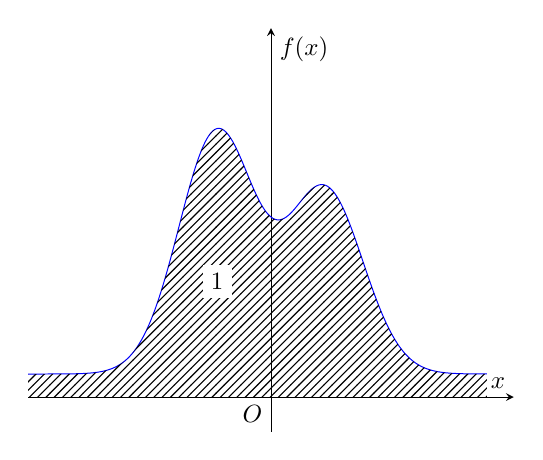
\begin{tikzpicture}[scale = 0.9]
  \begin{axis}[clip=false,xmin=-4.5,xmax=4.5,ymin=-0.15,ymax=1.6,ticks=none,axis lines=middle,smooth,xlabel={$x$}, ylabel={$f(x)$}]
    \addplot[draw=blue,domain=-4.5:4,samples=200] {1.05*e^(-(x+1)^2) + 0.8*e^(-(x-1)^2) + 0.1};
    \addplot+[draw=none,mark=none,domain=-4.5:4,samples=100,%
              pattern=north east lines]%
              {1.05*e^(-(x+1)^2) + 0.8*e^(-(x-1)^2) + 0.1}
              \closedcycle;
    \node[fill=white] at (-1,0.5) {$1$};
    \node[below left] at (0,0) {$O$};
  \end{axis}
\end{tikzpicture}

  \end{subfigure}
  \begin{subfigure}[t]{0.48\linewidth}
    \centering
      \input{figure/2_cdf_section.tex}
  \end{subfigure}
  \caption{概率密度性质}
  \label{概率密度性质}
\end{figure}

\paragraph{}
由\textbf{性质4}在$f(x)$的连续点$x$处有

\begin{align}
  \label{f(x)连续性质}
  \begin{split}
    f(x) =&\; \lim_{\Delta x \to 0^+}\frac{F(x+\Delta x) - F(x)}{\Delta x} \\
    =&\; \lim_{\Delta x \to 0^+}\frac{P\{x < X \leq x + \Delta x\}}{\Delta x}.
  \end{split}
\end{align}

\paragraph{}
由 \eqref{f(x)连续性质} 式知道,若不计高阶无穷小,有

\begin{equation}
  P\{x < X \leq x + \Delta x\} \approx f(x)\Delta x.
\end{equation}

这表示$X$落在小区间$(x, x+\Delta x]$上的概率近视地等于$f(x)\Delta x$.

\paragraph{}
对于连续型随机变量$X$来说,它取任一指定实数值$a$的概率均为$0$,即$P\{X=a\}=0$,因此可以不必区分该区间是开区间或闭区间:

\begin{equation}
  P\{a < X \leq b\} = P\{a \leq X \leq b\} = P\{a < X < b\}.
\end{equation}

\paragraph{}
下面介绍三种重要的连续型随机变量。

\subsubsection{均匀分布}
\paragraph{}
若连续型随机变量$X$具有概率密度

\begin{equation}
  f(x) = \left\{ \begin{array}{ll}
    \frac{1}{b-a}, & a<x<b, \\
    0, & \textbf{\small 其它},
  \end{array}\right.
\end{equation}

则称$X$在区间$(a,b)$上服从\textbf{均匀分布}。记为$X \sim U(a,b)$

\paragraph{}
对于任一长度$l$的子区间$(c, c+l), a \leq c < c+l \leq b$,有

\begin{equation}
  P\{c < X \leq c+l\} = \int_c^{c+l}f(x)dx = \int_c^{c+l}\frac{1}{b-a}dx=\frac{l}{b-a}.
\end{equation}

\paragraph{}
由 \eqref{连续型随机变量的分布函数} 式得$X$的分布函数为:

\begin{equation}
  F(x) = \left\{ \begin{array}{ll}
    0, & x < a, \\
    \frac{x-a}{b-a}, & a \leq x < b, \\
    1, & x \geq b.
  \end{array} \right.
\end{equation}

\paragraph{}
$f(x)$及$F(x)$的图形分别为:

\begin{figure}[h]
\centering
  %------- 第1行 -------
  \begin{subfigure}[t]{0.48\linewidth}
    \centering
      \input{figure/2_uniform.tex}
  \end{subfigure}
  \begin{subfigure}[t]{0.48\linewidth}
    \centering
      \input{figure/2_uniform_cumulative.tex}
  \end{subfigure}
  \caption{均匀分布的概率密度及其分布函数}
  \label{均匀分布的概率密度及其分布函数}
\end{figure}

\subsubsection{指数分布}
\paragraph{}

\subsubsection{正态分布}
\paragraph{}

\subsection{随机变量的函数的分布}
\paragraph{}

  \section{多维随机变量及其分布}
    \subsection{二维随机变量}
\subsubsection{二维随机变量}
\paragraph{}
设$E$是一个随机试验,它的样本空间是$S=\{e\}$,设$X=X(e)$和$Y=Y(e)$是定义在$S$上的随机变量,由它们构成的一个向量$(X,Y)$,叫做\textbf{二维随机向量}或\textbf{二维随机变量}

\begin{figure}[h]
\centering
% 二维随机变量
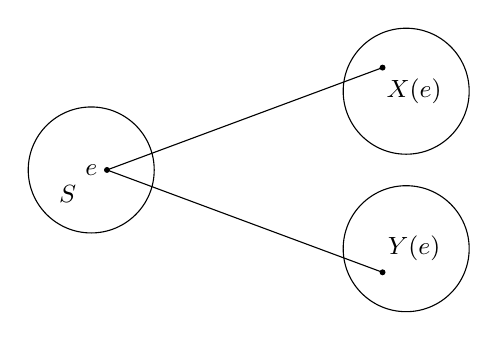
\begin{tikzpicture}
  % S = {e}
  \draw (0,0) circle [radius=0.8];
  \node at (0,0) {\small $e$};
  \node at (-0.3,-0.3) {\small $S$};

  % X = X(e)
  \draw (4,1) circle [radius=0.8];
  \node at (4.1,1) {\small $X(e)$};

  % Y = Y(e)
  \draw (4,-1) circle [radius=0.8];
  \node at (4.1,-1) {\small $Y(e)$};

  % 端点
  \draw [fill] (0.2,0) circle [radius=0.03];
  \draw [fill] (3.7,1.3) circle [radius=0.03];
  \draw [fill] (3.7,-1.3) circle [radius=0.03];
  % 连线
  \draw [thin] (0.2,0) -- (3.7,1.3);
  \draw [thin] (0.2,0) -- (3.7,-1.3);

\end{tikzpicture}

\caption{二维随机变量}
\label{二维随机变量}
\end{figure}

\paragraph{}
\textbf{定义\;}设$(X,Y)$是二维随机变量,对于任意实数$x,y$,二元函数:

\begin{equation}
  F(x,y) = P\{(X \leq x) \cap (Y \leq y) \} \xlongequal{\text{记成}} P\{X \leq x, Y \leq y\}
\end{equation}

称为二维随机变量$(X,Y)$的\textbf{分布函数},或称为随机变量$X$和$Y$的\textbf{联合分布函数}。

\paragraph{}

\begin{figure}[h]
\centering
  %------- 第1行 -------
  \begin{subfigure}[t]{0.48\linewidth}
    \centering
      % 二维随机变量的分布函数图解
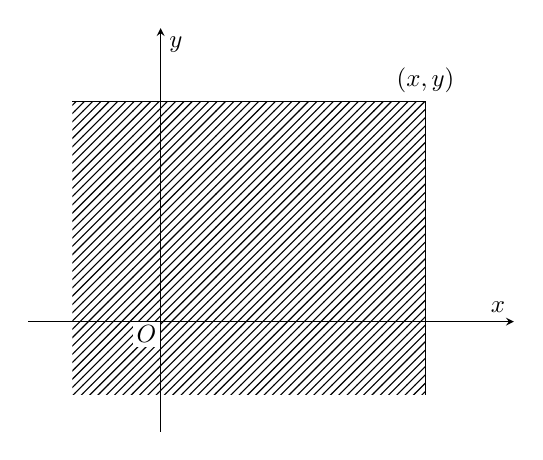
\begin{tikzpicture}[scale = 0.9]
  \begin{axis}[clip=false,xmin=-1.5,xmax=4,ymin=-1.5,ymax=4,ticks=none,axis lines=middle,smooth,xlabel={$x$}, ylabel={$y$}]
    \draw (-1,3) -- (3,3) -- (3,-1);
    \fill[pattern=north east lines] (-1,-1) rectangle (3,3);
    \node[above] at (3,3) {$(x,y)$};
    \node[below left,fill=white, inner sep=1.5] at (0,0) {$O$};
  \end{axis}
\end{tikzpicture}

    \subcaption{分布函数图解}
  \end{subfigure}
  \begin{subfigure}[t]{0.48\linewidth}
    \centering
      % 二维随机变量的分布函数图解,矩形域
\begin{tikzpicture}[scale = 0.9]
  \begin{axis}[clip=false,xmin=-1.5,xmax=4,ymin=-1.5,ymax=4,ticks=none,axis lines=middle,smooth,xlabel={$x$}, ylabel={$y$}]
    % 矩形
    \draw (1,1) rectangle (3,3);
    % 矩形辅助线
    \draw[dashed] (0,3) -- (1,3);
    \node[left] at (0,3) {$y_2$};
    \draw[dashed] (0,1) -- (1,1);
    \node[left] at (0,1) {$y_1$};
    % 矩形辅助线
    \draw[dashed] (1,1) -- (1,0);
    \node[below] at (1,0) {$x_1$};
    \draw[dashed] (3,1) -- (3,0);
    \node[below] at (3,0) {$x_2$};
    % (x,y)
    \node[above] at (3,3) {$(x,y)$};
    % 原点
    \node[below left, inner sep=1.5] at (0,0) {$O$};
  \end{axis}
\end{tikzpicture}

    \subcaption{矩形域图解}
  \end{subfigure}
  \caption{分布函数图解}
  \label{二维随机变量的分布函数图解}
\end{figure}

\textbf{性质:\;}

\begin{enumerate}
  \item $F(x,y)$是变量$x$和$y$的不减函数,即对于任意固定的$y$,当$x_2 > x_1$时$F(x_2,y)\geq F(x_1,y)$;对于任意固定的$x$,当$y_2 > y_1$时$F(x,y_2) \geq F(x,y_1)$。
  \item $0 \leq F(x,y) \leq 1$,且
  \begin{enumerate}
    \item 对于任意固定的$y, F(-\infty,y)=0$,
    \item 对于任意固定的$x, F(x,-\infty)=0$,
    \item $F(-\infty, -\infty) = 0, F(\infty,\infty)=1$。
  \end{enumerate}
  \item $F(x+0,y)=F(x,y),F(x,y+0)=F(x,y)$,即$F(x,y)$关于$x$右连续,关于$y$也右连续。
  \item 对于任意$(x_1,y_1), (x_2,y_2), x_1 < x_2, y_1 < y_2$,下述不等式成立:
  \begin{equation}
    F(x_2,y_2) - F(x_2,y_1) + F(x_1,y_1) - F(x_1,y_2) \geq 0.
  \end{equation}
  参考\linkref[二维随机变量的分布函数图解]{矩形域图解}。
\end{enumerate}

\subsubsection{离散型的随机变量}
\paragraph{}
如果二维随机变量$(X,Y)$全部可能取到的值是\textbf{有限对}或\textbf{可列无限多对},则称$(X,Y)$是\textbf{离散型的随机变量}。
\paragraph{}
设二维离散型随机变量$(X,Y)$所有可能取的值为$(x_i,y_j),i,j=1,2,\cdots,$记$P\{X=x_i,Y=y_j\}=p_{ij},i,j=1,2,\cdots,$则由概率的定义有

\begin{equation}
  p_{ij} \geq 0, \sum_{i=1}^\infty\sum_{j=1}^\infty p_{ij} = 1.
\end{equation}

\paragraph{}
我们称$P\{X=x_i,Y=y_j\}=p_{ij},i,j=1,2,\cdots$为二维离散型随机变量$(X,Y)$的\textbf{分布律},或随机变量$X$和$Y$的\textbf{联合分布律}。

\paragraph{}
我们也能用表格来表示$X$和$Y$的联合分布律:

\bgroup
\def\arraystretch{1.5}
\setlength\tabcolsep{0.8cm}
\begin{figure}[H]
\centering
  \begin{tabular}{c|ccccc}
    \hline
    \backslashbox{$Y$}{$X$} & $x_1$ & $x_2$ & $\cdots$ & $x_i$ & $\cdots$ \\
    \hline
    $y_1$ & $p_{11}$ & $p_{21}$ & $\cdots$ & $p_{i1}$ & $\cdots$ \\
    \hline
    $y_2$ & $p_{12}$ & $p_{22}$ & $\cdots$ & $p_{i2}$ & $\cdots$ \\
    \hline
    $\vdots$ & $\vdots$ & $\vdots$ &  & $\vdots$ & \\
    \hline
    $y_j$ & $p_{1j}$ & $p_{2j}$ & $\cdots$ & $p_{ij}$ & $\cdots$ \\
    \hline
    $\vdots$ & $\vdots$ & $\vdots$ &  & $\vdots$ & \\
    \hline
  \end{tabular}
\end{figure}
\egroup

\paragraph{}
将$(X,Y)$看成一个随机点的坐标,由图\figureref{二维随机变量的分布函数图解}知道离散型随机变量$X$和$Y$的\textbf{联合分布函数}为:

\begin{equation}
  \label{离散型随机变量的联合分布函数}
  F(x,y) = \sum_{x_i \leq  x} \sum_{y_j \leq y} p_{ij},
\end{equation}

其中和式是对一切满足$x_i \leq x, \; y_j \leq y$的$i,j$来求和的。

\subsubsection{连续型的随机变量}
\paragraph{}
对于二维变量$(X,Y)$的分布函数$F(x,y)$,如果存在非负的函数$f(x,y)$使对于任意$x,y$有

\begin{equation}
  F(x,y)=\int_{-\infty}^y\int_{-\infty}^xf(u,v)dudv,
\end{equation}

则称$(X,Y)$是\textbf{连续型的二维随机变量},函数$f(x,y)$称为二维随机变量$(X,Y)$的\textbf{概率密度},或称为随机变量$X$和$Y$的\textbf{联合概率密度}。

\paragraph{}
概率密度$f(x,y)$具有以下性质:
\begin{enumerate}
  \item $f(x,y) \geq 0$
  \item $\int_{-\infty}^\infty\int_{-\infty}^\infty f(x,y)dxdy=F(\infty,\infty)=1$
  \item 设$G$是$xOy$平面上的区域,点$(X,Y)$落在$G$内的概率为
  \begin{equation}
    P\{(X,Y)\in G\} = \iint\limits_G f(x,y)dxdy
  \end{equation}
  \item 若$f(x,y)$在点$(x,y)$连续,则有
  \begin{equation}
    \frac{\partial^2F(x,y)}{\partial x\partial y} = f(x,y)
  \end{equation}
\end{enumerate}

\subsubsection{$n$维随机变量}
\paragraph{}
一般,设$E$是一个随机试验,它的样本空间是$S=\{e\}$,设$X_1=X_1(e), X_2=X_2(e),\cdots,X_n=X_n(e)$是定义在$S$上的随机变量,由它们构成的一个$n$维向量$(X_1,X_2,\cdots,X_n)$叫做\textbf{$n$维随机向量}或\textbf{$n$维随机变量}。
\paragraph{}
对于任意$n$个实数$x_1,x_2,\cdots,x_n$,$n$元函数
\begin{equation}
  F(x_1,x_2,\cdots,x_n)=P\{X_1 \leq  x_1, X_2 \leq x_2, \cdots, X_n \leq x_n\}
\end{equation}
称为$n$维随机变量$(X_1,X_2,\cdots,X_n)$的\textbf{分布函数}或随机变量$X_1,X_2,\cdots,X_n$的\textbf{联合分布函数}。它具有类似于二维随机变量的分布函数的性质。

\subsection{边缘分布}
\subsubsection{边缘分布}
\paragraph{}
二维随机变量$(X,Y)$作为一个整体,具有分布函数$F(x,y)$,而$X$和$Y$都是随机变量,各自也有分布函数,将它们分别记为$F_X(x), F_Y(y)$,依次称为二维随机变量$(X,Y)$关于$X$和关于$Y$的\textbf{边缘分布函数},边缘分布函数可以由$(X,Y)$的分布函数$F(x,y)$所确定,事实上,
\begin{equation}
  F_x(x) = P\{X\leq x\} = P\{X\leq x, Y < \infty\} = F(x,\infty),
\end{equation}
即
\begin{equation}
  \label{F_X(x)边缘分布}
  F_X(x)=F(x,\infty).
\end{equation}
就是说,只要在函数$F(x,y)$中令$y \to \infty$就能得到$F_X(x)$,同理
\begin{equation}
  F_Y(y) = F(\infty,y).
\end{equation}

\subsubsection{离散型随机变量}
\paragraph{}
对于离散型随机变量,由\eqref{离散型随机变量的联合分布函数}、\eqref{F_X(x)边缘分布}式可得
\begin{equation}
  F_X(x)=F(x,\infty)=\sum_{x_i \leq x}\sum_{j=1}^\infty p_{ij}.
\end{equation}

与第二章\eqref{X的分布函数}式比较,知道$X$的分布律为

\begin{equation}
  P\{X=x_i\} = \sum_{j=1}^\infty p_{ij}, \; i = 1, 2, \cdots.
\end{equation}

同样,$Y$的分布律为

\begin{equation}
  P\{Y=y_i\} = \sum_{i=1}^\infty p_{ij}, \; j = 1, 2, \cdots.
\end{equation}

记
\begin{align}
\begin{split}
  p_{i\bigcdot} &= \sum_{j=1}^\infty p_{ij} = P\{X=x_i\}, \; i = 1,2,\cdots, \\
  p_{\bigcdot j} &= \sum_{i=1}^\infty p_{ij} = P\{Y=y_j\}, \; j = 1,2,\cdots,
\end{split}
\end{align}

分别称$p_{i\bigcdot}(i=1,2,\cdots)$和$p_{\bigcdot j}(j=1,2,\cdots)$为$(X,Y)$关于$X$和关于$Y$的\textbf{边缘分布律}

\subsubsection{连续型随机变量}
\paragraph{}
对于连续型随机变量$(X,Y)$,设它的概率密度为$f(x,y)$,由于
\begin{equation}
  F_X(x) = F(x,\infty)=\int_{-\infty}^x\Big[\int_{-\infty}^\infty f(x,y)dy\Big]dx,
\end{equation}
由第二章\eqref{连续型随机变量的分布函数}式知道,$X$是一个连续型随机变量,且其概率密度为
\begin{equation}
  f_X(x) = \int_{-\infty}^\infty f(x,y)dy.
\end{equation}
同样,$Y$也是一个连续型随机变量,其概率密度为
\begin{equation}
  f_Y(y) = \int_{-\infty}^\infty f(x,y)dy.
\end{equation}
分别称$f_X(x),f_Y(y)$为$(X,Y)$关于$X$和关于$Y$的\textbf{边缘概率密度}。

\paragraph{}
平时将边缘分布律写在联合分布律表格的边缘上,这就是“边缘分布律”的由来,例如:

\bgroup
\def\arraystretch{1.5}
\setlength\tabcolsep{0.5cm}
\begin{figure}[H]
\centering
  \begin{tabular}{c|cccc|c}
    \hline
    \backslashbox{$F$}{$D$} & $1$ & $2$ & $3$ & $4$ & $P\{F=j\}$ \\
    \hline
    $0$ & $\frac{1}{10}$ & $0$ & $0$ & $0$ & $\frac{1}{10}$ \\
    $1$ & $0$ & $\frac{4}{10}$ & $\frac{2}{10}$ & $\frac{1}{10}$ & $\frac{7}{10}$ \\
    $2$ & $0$ & $0$ & $0$ & $\frac{2}{10}$ & $\frac{2}{10}$ \\
    \hline
    $P\{D=i\}$ & $\frac{1}{10}$ & $\frac{4}{10}$ & $\frac{2}{10}$  & $\frac{3}{10}$ & $1$ \\
    \hline
  \end{tabular}
\end{figure}
\egroup

即有边缘分布律
\bgroup
\def\arraystretch{2}
\setlength\tabcolsep{0.5cm}
\begin{figure}[H]
\centering
%------- 第1行 -------
\begin{subfigure}[t]{0.48\linewidth}
  \centering
    \begin{tabular}{c|cccc}
      \hline
      $D$ & $1$ & $2$ & $3$ & $4$ \\
      \hline
      $p_k$ & $\frac{1}{10}$ & $\frac{4}{10}$ & $\frac{2}{10}$ & $\frac{3}{10}$ \\
      \hline
    \end{tabular}
\end{subfigure}
\begin{subfigure}[t]{0.48\linewidth}
  \centering
    \begin{tabular}{c|ccc}
      \hline
      $F$ & $0$ & $1$ & $2$ \\
      \hline
      $p_k$ & $\frac{1}{10}$ & $\frac{7}{10}$ & $\frac{2}{10}$ \\
      \hline
    \end{tabular}
\end{subfigure}
\end{figure}
\egroup

\subsection{条件分布}
\subsubsection{离散型随机变量}
\paragraph{}
\textbf{定义\;}设$(X,Y)$是二维离散型随机变量,对于固定的$j$,若$P\{Y=y_j\}>0$,则称
\begin{equation}
  P\{X=x_i|Y=y_j\} = \frac{P\{X=x_i,Y=y_j\}}{P\{Y=y_j\}} = \frac{p_{ij}}{p_{\bigcdot j}}, \; i = 1,2,\cdots
\end{equation}
为在$Y=y_j$条件下随机变量$X$的\textbf{条件分布律}。同样,可得到$Y$的条件分布律。

\subsubsection{连续型随机变量}
\paragraph{}
\textbf{定义\;}设二维随机变量$(X,Y)$的概率密度为$f(x,y), (X,Y)$关于$Y$的边缘概率密度为$f_Y(y)$,若对于固定的$y, f_Y (y)>0$,则称$\frac{f(x,y)}{f_Y(y)}$为在$Y=y$的条件下$X$的\textbf{条件概率密度},记为
\begin{equation}
  f_{X|Y}(x|y) = \frac{f(x,y)}{f_Y(y)}.
\end{equation}

称$\int_{-\infty}^x f_{X|Y}(x|y)dx = \int_{-\infty}^x \frac{f(x,y)}{f_Y(y)}dx$为在$Y=y$的条件下$X$的条件分布函数,记为$P\{X \leq  x | Y = y\}$或$F_{X|Y}(x|y)$,即

\begin{equation}
  F_{X|Y}(x|y) = P\{X \leq x | Y = y\}=\int_{-\infty}^x\frac{f(x,y)}{f_Y(y)}dx.
\end{equation}

类似地,可以定义$f_{Y|X}(y|x)=\frac{f(x,y)}{f_X(x)}$和$F_{Y|X}(y|x)=\int_{-\infty}^y\frac{f(x,y)}{f_X(x)}dy.$

\subsection{相互独立的随机变量}
\paragraph{}
\textbf{定义\;}设$F(x,y)$及$F_X(x),F_Y(y)$分别是二维随机变量$(X,Y)$的分布函数及边缘分布函数。若对于所有$x,y$有
\begin{equation}
  P\{X \leq x, Y \leq y\} = P\{X \leq x\}P\{Y \leq y\},
\end{equation}
即
\begin{equation}
  \label{二维随机变量的相互独立性}
  F(x,y) = F_X(x)F_Y(y),
\end{equation}
则称随机变量$X$和$Y$是\textbf{相互独立的}。

\paragraph{}
设$(X,Y)$是连续型随机变量,$f(x,y), f_X(x), f_Y(y)$分别为$(X,Y)$的概率密度和边缘概率密度,则$X$和$Y$相互独立的条件\eqref{二维随机变量的相互独立性}等价于
\begin{equation}
  f(x,y)=f_X(x)f_Y(y)
\end{equation}
在平面上几乎处处成立。

\paragraph{}
当$(X,Y)$是离散型随机变量时,$X$和$Y$相互独立的条件\eqref{二维随机变量的相互独立性}式等价于:对于$(X,Y)$的所有可能取的值$(x_i,y_j)$有
\begin{equation}
  P\{X=x_i,Y=y_j\} = P\{X=x_i\}P\{Y=y_j\}.
\end{equation}

\textbf{定理\;}设$(X_1, X_2, \cdots, X_m)$和$(Y_1, Y_2, \cdots, Y_n)$相互独立,则$X_i(i=1,2, \cdots, m)$和$Y_j(j=1,2, \cdots, n)$相互独立,又若$h,g$是连续函数,则$h(X_1,X_2, \cdots, X_m)$和$g(Y_1, Y_2, \cdots, Y_n)$相互独立。

\subsection{两个随机变量的函数的分布}
\paragraph{}
【TODO】

  \section{随机变量的数字特征}
    \subsection{数学期望}
\subsubsection{例子}
\paragraph{}
\textbf{例子\;}一射手进行打靶练习,规定射入区域$e_2$得2分,射入区域$e_1$得1分,脱靶,即射入区域$e_0$,得0分。射手一次射击得分数$X$是一个随机变量。设$X$的分布律为

\begin{equation*}
  P\{X=k\}=p_k, \; k = 0,1,2.
\end{equation*}

\begin{figure}[H]
\centering
  % 打靶练习
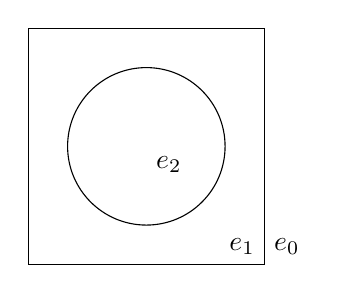
\begin{tikzpicture}
  \draw (-1.5,-1.5) rectangle (1.5,1.5);
  \draw (0,0) circle [radius=1];

  \node[below right] at (0,0) {$e_2$};
  \node[above left] at (1.5,-1.5) {$e_1$};
  \node[above right] at (1.5,-1.5) {$e_0$};
\end{tikzpicture}

  \caption{打靶练习}
  \label{打靶练习}
\end{figure}

\paragraph{}
现在射击$N$次,其中得0分的有$a_0$次,得1分的有$a_1$次,得2分的有$a_2$次,$a_0+a_1+a_2=N$。他射击$N$次得分的总和为$a_0 \times 0 + a_1 \times 1 + a_2 \times 2$。于是平均一次射击的得分数为
\begin{equation*}
  \frac{a_0 \times 0 + a_1 \times 1 + a_2 \times 2}{N} = \sum_{k=0}^2 k \frac{a_k}{N}.
\end{equation*}

\paragraph{}
这里,$\displaystyle \frac{a_k}{N}$是事件$\{X=k\}$的频率。当$N$很大时,$\displaystyle \frac{a_k}{N}$在一定意义下接近于事件$\{X=k\}$的概率$p_k$。就是说,在试验次数很大时,随机变量$X$的观察值的算术平均$\displaystyle \sum_{k=0}^2 k \frac{a_k}{N}$在一定意义下接近于$\displaystyle \sum_{k=0}^2 kp_k$。我们称$\displaystyle \sum_{k=0}^2 kp_k$为随机变量$X$的数学期望或均值。

\subsubsection{定义}
\paragraph{}
\textbf{定义\;}设离散型随机变量$X$的分布律为

\begin{equation*}
  P\{X=x_k\} = p_k, \; k = 1,2,\cdots.
\end{equation*}

若级数
\begin{equation*}
  \sum_{k=1}^\infty x_k p_k
\end{equation*}

绝对收敛,则称级数$\displaystyle \sum_{k=1}^\infty x_k p_k$的和为随机变量$X$的\textbf{数学期望},记为$E(X)$。即

\begin{equation}
  \label{离散型随机变量的数学期望}
  E(X) = \sum_{k=1}^\infty x_k p_k
\end{equation}

\paragraph{}
设连续型随机变量$X$的概率密度为$f(x)$,若积分

\begin{equation*}
  \int_{-\infty}^\infty xf(x)dx
\end{equation*}

绝对收敛,则称积分$\displaystyle \int_{-\infty}^\infty xf(x)dx$的值为随机变量$X$的\textbf{数学期望},记为$E(X)$。即

\begin{equation}
  \label{随机型随机变量的数学期望}
  E(X)=\int_{-\infty}^\infty xf(x)dx
\end{equation}

\paragraph{}
数学期望简称\textbf{期望},又称为\textbf{均值}。

\subsubsection{定理}
\paragraph{}
\textbf{定理\;}设$Y$是随机变量$X$的函数:$Y=g(X)$($g$是连续函数)。
\begin{enumerate}
  \item 如果$X$是离散型随机变量,它的分布律为$P\{X=x_k\}=p_k, \; k = 1,2,\cdots,$若$\displaystyle \sum_{k=1}^\infty g(x_k)p_k$绝对收敛,则有
  \begin{equation}
    E(Y)=E[g(X)]=\sum_{k=1}^\infty g(x_k)p_k.
  \end{equation}
  \item 如果$X$是连续型随机变量,它的概率密度为$f(x)$,若$\displaystyle \int_{-\infty}^\infty g(x)f(x)dx$绝对收敛,则有
  \begin{equation}
    E(Y) = E[g(X)] = \int_{-\infty}^\infty g(x)f(x)dx.
  \end{equation}
\end{enumerate}

\paragraph{}
定理的重要意义在于当我们求$E(Y)$时,不必算出$Y$的分布律或概率密度,而只需利用$X$的分布律或概率密度就可以了。

\subsubsection{性质}
\paragraph{}
\begin{enumerate}
  \item 设$C$是常数,则有$E(C)=C$。
  \item 设$X$是一个随机变量,$C$是常数,则有$E(CX)=CE(X)$。
  \item 设$X,Y$是两个随机变量,则有$E(X+Y)=E(X) + E(Y)$。这一性质可以推广到任意有限个随机变量之和的情况。
  \item 设$X,Y$是\textbf{相互独立的}随机变量,则有$E(XY)=E(X)E(Y)$。这一性质可以推广到任意有限个\textbf{相互独立的}随机变量之积的情况。
\end{enumerate}

\subsection{方差}
\subsubsection{例子}
\paragraph{}
例如,有一批灯泡,知其平均寿命是$E(X)=1\,000$(小时)。仅由这一指标我们还不能判断这批灯泡的质量好坏。还需进一步考察灯泡寿命$X$与其均值$E(X)=1\,000$的\textbf{偏离程度}。若偏离程度较小,表示质量比较稳定。容易看到

\begin{equation*}
  E\{|X-E(X)|\}
\end{equation*}

能度量随机变量与其均值$E(X)$的偏离程度。但由于上式带有绝对值,运算不方便,为运算方便起见,通常用量
\begin{equation*}
  E\{[X-E(X)]^2\}
\end{equation*}
来度量随机变量$X$与其均值$E(X)$的偏离程度。

\subsubsection{定义}
\paragraph{}
\textbf{定义\;}设$X$是一个随机变量,若$E\{[X-E(X)]^2\}$存在,则称$E\{[X-E(X)]^2\}$为$X$的\textbf{方差},记为$D(X)$或$Var(X)$,即
\begin{equation}
  D(X)=Var(X)=E\{[X-E(X)]^2\}.
\end{equation}

\paragraph{}
在应用上还引入量$\sqrt{D(X)}$,记为$\sigma(X)$,称为\textbf{标准差}或\textbf{均方差}。

\paragraph{}
$D(X)$是刻画$X$取值分散程度的一个量,它是衡量$X$取值分散程度的一个尺度。

\paragraph{}
由定义知,方差是随机变量$X$的函数$g(X)=(X-E(X))^2$的数学期望。于是对于离散型随机变量,按\eqref{离散型随机变量的数学期望}式有:
\begin{equation}
  D(X) = \sum_{k=1}^\infty[x_k - E(X)]^2p_k,
\end{equation}
其中$P\{X=x_k\}=p_k,\;k=1,2,\cdots$是$X$的分布律。

\paragraph{}
对于连续型随机变量,按\eqref{随机型随机变量的数学期望}式有:
\begin{equation}
  D(X) = \int_{-\infty}^\infty [x - E(X)]^2f(x)dx,
\end{equation}
其中$f(x)$是$X$的概率密度。

\paragraph{}
随机变量$X$的方差可按下列公式计算:
\begin{equation}
  D(X)=E(X^2)-[E(X)]^2.
\end{equation}

\paragraph{}
设随机变量$X$具有数学期望$E(X)=\mu$,方差$D(X)=\sigma^2 \neq 0$。记
\begin{equation}
  X^* = \frac{X-\mu}{\sigma},
\end{equation}
则
\begin{align*}
  E(X^*) =&\, \frac{1}{\sigma}E(X-\mu)=\frac{1}{\sigma}[E(X)-\mu] = 0; \\
  D(X^*) =&\, E(X^{*2}) - [E(X^*)]^2 = E\Big[\Big(\frac{X-\mu}{\sigma}\Big)^2\Big] \\
         =&\, \frac{1}{\sigma^2}E[(X-\mu)^2]=\frac{\sigma^2}{\sigma^2} = 1
\end{align*}
即$\displaystyle X^* = \frac{X-\mu}{\sigma}$ 的数学期望为$0$,方差为$1$。$X^*$称为$X$的\textbf{标准化变量}。

\subsubsection{性质}
\paragraph{}
性质
\begin{enumerate}
  \item 设$C$是常数,则$D(C)=0$.
  \item 设$X$是随机变量,$C$是常数,则有
  \begin{equation*}
    D(CX) = C^2D(X), \; D(X+C)=D(X).
  \end{equation*}
  \item 设$X,Y$是两个随机变量,则有
  \begin{equation*}
    D(X+Y) = D(X) + D(Y) + 2E\{(X-E(X))(Y-E(Y))\}.
  \end{equation*}
  特别,若$X,Y$相互独立,则有
  \begin{equation*}
    D(X+Y) = D(X) + D(Y).
  \end{equation*}
  \item $D(X)=0$的充要条件是$X$以概率$1$取常数$E(X)$,即
  \begin{equation*}
    P\{X=E(X)\} = 1.
  \end{equation*}
\end{enumerate}

\subsubsection{定理}
\paragraph{}
\textbf{定理\;}设随机变量$X$具有数学期望$E(X)=\mu$,方差$D(X)=\sigma^2$,则对于任意正数$\varepsilon$,不等式
\begin{equation}
  P\{|X-\mu| \geq \varepsilon \} \leq \frac{\sigma^2}{\varepsilon^2}
\end{equation}
成立。

\paragraph{}
这一不等式称为\textbf{切比雪夫(Chebyshev)不等式}。

\paragraph{}
\textbf{意义\;}该不等式给出了在随机变量的分布未知,而只知道$E(X)$和$D(X)$的情况下估计概率$P\{|X-E(X)|<\varepsilon\}$的界限。
\paragraph{}
这个估计是比较粗糙的,如果已经知道随机变量的分布时,那么所需求的概率可以确切地计算出来,也就没有必要利用这一不等式来作估计了。

\subsection{协方差及相关系数}
\paragraph{}

\subsection{矩、协方差矩阵}
\paragraph{}

\end{document}
